% --------------------------------------------------------------------
% Technical Documentation
% Marco Müller
% --------------------------------------------------------------------

\documentclass[11pt, a4paper, listof=numbered, captions=tableheading, headinclude, table, xcdraw]{scrreprt}
\usepackage[utf8]{inputenc}
\usepackage{babel}
\usepackage{tikz}
\usepackage{epigraph}
%\usepackage[T1]{fontenc}
\usepackage{xcolor}
\usepackage{amsmath}
\usepackage{textgreek}
\usepackage[LGRgreek]{mathastext}
\usepackage{array}
\usepackage{color}
\usepackage{graphicx}
\usepackage{float}
\usepackage{helvet}
\usepackage{scrhack}
\usepackage{makecell}
\usepackage{dirtree}
\renewcommand{\familydefault}{\sfdefault}

\setcounter{secnumdepth}{4} % give subsubsection numbers

\setlength{\emergencystretch}{\hsize}
\tolerance=9999

\newcounter{divide}

% für referenziertes Inhaltsverzeichnis
\usepackage[hidelinks, hypertexnames=false]{hyperref}

\usepackage{chngcntr}
\counterwithin*{chapter}{divide}

\renewcommand\epigraphflush{flushright}
\renewcommand\epigraphsize{\normalsize}
\setlength\epigraphwidth{0.7\textwidth}

\definecolor{titlepagecolor1}{cmyk}{.82,.24,0,.11}
\definecolor{titlepagecolor}{cmyk}{0,.33,.98,.2}

\DeclareFixedFont{\titlefont}{T1}{ppl}{b}{it}{0.5in}

\setlength{\parindent}{0pt}


% Seitenränder festlegen
\usepackage[top=1.5cm,bottom=1.5cm,right=2cm,left=2cm,includeheadfoot]{geometry}

% ---------------------------------------
% Titeldefinition
\newcommand{\Titel}{Documentation\\\vspace{.5mm}Plantomation V1.0}
\newcommand{\Caption}{Automatic Plant Watering System}
\newcommand{\SignateAuthor}{\textit{Made with \LaTeX}}
\newcommand{\Stand}{\textit{Compiled: \today}}
% Sonstiges in titel.ltx und titel-meta.ltx
% ---------------------------------------

% Kopf- und Fußzeile
\usepackage[automark]{scrlayer-scrpage}

% --------------------------------------------------------------------
% Titelblatt
% --------------------------------------------------------------------

\makeatletter                       
\def\printauthor{         
    {\large \@author}}              
\makeatother
\author{
    Synthron \\ 
    \vspace*{12pt}
    \texttt{admin@synthron.de}
    }

\renewcommand\epigraphflush{flushright}
\renewcommand\epigraphsize{\normalsize}
\setlength\epigraphwidth{0.7\textwidth}

\definecolor{Green}{gray}{0.55}

\newcommand\anglei{-45}
\newcommand\angleii{-45}
\newcommand\angleiii{-225}
\newcommand\angleiv{135}

\newcommand\titlepagedecoration{%
\begin{tikzpicture}[remember picture,overlay,shorten >= -10pt]

\coordinate (aux1) at ([yshift=-15pt]current page.north east);
\coordinate (aux2) at ([yshift=-410pt]current page.north east);
\coordinate (aux3) at ([xshift=-4.5cm]current page.north east);
\coordinate (aux4) at ([yshift=-150pt]current page.north east);

\begin{scope}[titlepagecolor!40,line width=12pt,rounded corners=12pt]
\draw
  (aux1) -- coordinate (a)
  ++(225:5) --
  ++(-45:5.1) coordinate (b);
\draw[shorten <= -10pt]
  (aux3) --
  (a) --
  (aux1);
\draw[opacity=0.6,titlepagecolor,shorten <= -10pt]
  (b) --
  ++(225:2.2) --
  ++(-45:2.2);
\end{scope}
\draw[titlepagecolor,line width=8pt,rounded corners=8pt,shorten <= -10pt]
  (aux4) --
  ++(225:0.8) --
  ++(-45:0.8);
\begin{scope}[titlepagecolor!70,line width=6pt,rounded corners=8pt]
\draw[shorten <= -10pt]
  (aux2) --
  ++(225:3) coordinate[pos=0.45] (c) --
  ++(-45:3.1);
\draw
  (aux2) --
  (c) --
  ++(135:2.5) --
  ++(45:2.5) --
  ++(-45:2.5) coordinate[pos=0.3] (d);   
\draw 
  (d) -- +(45:1);
\end{scope}
\end{tikzpicture}%
}
\newcommand\chapterdecoration{%
\begin{tikzpicture}[remember picture,overlay,shorten >= -10pt]
\coordinate (aux1) at ([yshift=-15pt]current page.north west);
\coordinate (aux2) at ([yshift=-310pt]current page.north west);
\coordinate (aux3) at ([xshift=4.5cm]current page.north west);
\coordinate (aux4) at ([yshift=-150pt]current page.north west);
\coordinate (aux5) at ([yshift=-535pt]current page.north west);
\coordinate (aux6) at ([yshift=-660pt]current page.north west);
\coordinate (aux7) at ([yshift=-630pt]current page.north west);
\coordinate (aux8) at ([xshift=-16.5cm]current page.south east);
\renewcommand\anglei{-135}
\renewcommand\angleii{135}
\renewcommand\angleiii{-45}
\renewcommand\angleiv{45}



\begin{scope}[titlepagecolor1!70,line width=6pt,rounded corners=8pt]
\draw[shorten <= -10pt]
  (aux2) --
  ++(\angleiii:3) coordinate[pos=0.4] (d) --
  ++(\anglei:3.1);

\draw
  (d) --
  ++(\angleiii:.1) --
 ++(\angleiii:1.7) --
  ++(\anglei:1.5) --
++(\angleiii:2.5) --
++(\anglei:2.5) --
++(\angleii:2) --
++(\angleiii:1.3) --
++(\anglei:1.3) 
 
coordinate[pos=0.3] (c); 
\begin{scope}[titlepagecolor1!40,line width=12pt,rounded corners=12pt]
\draw
  (aux7) -- coordinate (a)
  ++(\angleiii:5) --
  ++(\anglei:5.1) coordinate (b);
\draw[shorten <= -10pt]
  
  (b) -- 
++(\angleiv:2.5) --
++(\angleiii:5) 
  (aux8);
\draw[opacity=0.6,titlepagecolor1,shorten <= -10pt]
  (aux5) --
  ++(\angleiii:2.2) --
  ++(\anglei:2.2);
\draw[titlepagecolor1,line width=8pt,rounded corners=8pt,shorten <= -10pt]
  (aux6) --
  ++(\angleiii:0.8) --
  ++(\anglei:0.8);
\end{scope}
  
\end{scope}
\end{tikzpicture}%
}

% Old Code for reference
%
%
%
%\newcommand\titlepagedecoration{
%\begin{tikzpicture}[remember picture,overlay,shorten >= -10pt]
%
%\coordinate (aux1) at ([yshift=-15pt]current page.north east);
%\coordinate (aux2) at ([yshift=-410pt]current page.north east);
%\coordinate (aux3) at ([xshift=-4.5cm]current page.north east);
%\coordinate (aux4) at ([yshift=-150pt]current page.north east);
%
%\begin{scope}[titlepagecolor!40,line width=12pt,rounded corners=12pt]
%\draw
%  (aux1) -- coordinate (a)
%  ++(225:5) --
%  ++(-45:5.1) coordinate (b);
%\draw[shorten <= -10pt]
%  (aux3) --
%  (a) --
%  (aux1);
%\draw[opacity=0.6,titlepagecolor,shorten <= -10pt]
%  (b) --
%  ++(225:2.2) --
%  ++(-45:2.2);
%\end{scope}
%\draw[titlepagecolor,line width=8pt,rounded corners=8pt,shorten <= -10pt]
%  (aux4) --
%  ++(225:0.8) --
%  ++(-45:0.8);
%\begin{scope}[titlepagecolor!70,line width=6pt,rounded corners=8pt]
%\draw[shorten <= -10pt]
%  (aux2) --
%  ++(225:3) coordinate[pos=0.45] (c) --
%  ++(-45:3.1);
%\draw
%  (aux2) --
%  (c) --
%  ++(135:2.5) --
%  ++(45:2.5) --
%  ++(-45:2.5) coordinate[pos=0.3] (d);   
%\draw 
%  (d) -- +(45:1);
%\end{scope}
%\end{tikzpicture}
%}

\begin{document}
\begin{titlepage}

\vspace*{2cm}
\noindent
\titlefont \Titel\par
\epigraph{\Caption}
{\SignateAuthor\\ \Stand}
\vspace*{2cm}
\centering{
\includegraphics[width=0.5\textwidth]{pictures/logo.png}}
\null\vfill
\vspace*{1cm}
\noindent
\hfill
\begin{minipage}{0.4\linewidth}
    \begin{flushright}
        \printauthor
    \end{flushright}
\end{minipage}
%
\begin{minipage}{0.02\linewidth}
    \rule{1pt}{80pt}
\end{minipage}
\titlepagedecoration
\chapterdecoration
\end{titlepage}


\KOMAoptions{parskip=half}
% --------------------------------------------------------------------
% Verzeichnisse
% --------------------------------------------------------------------

%\pagenumbering{Roman}
%\renewcommand{\thechapter}{\Roman{chapter}}
%
%\setcounter{tocdepth}{1} %Ausblenden von Subsections etc..
%\cohead[I Table Of Contents]{I Table Of Contents}
%\pagestyle{scrheadings}
%\tableofcontents 	\newpage
%\cohead[II List of Tables]{II List of Tables}
%\pagestyle{scrheadings}
%\listoftables 		\newpage
%\cohead[III List of Figures]{III List of Figures}
%\pagestyle{scrheadings}
%\listoffigures 		\newpage
%\pagenumbering{arabic}
%
%\stepcounter{divide}
%
%\renewcommand{\thechapter}{\arabic{chapter}}

% Kopfzeilen erst nach den Verzeichnissen

\lohead[\today]{\today}
\cohead[Plantomation]{Plantomation}
\rohead[Synthron]{Synthron}
\pagestyle{scrheadings}

% --------------------------------------------------------------------
% Ab hier der Inhalt
% --------------------------------------------------------------------

\chapter{Prelude}

Plantomation is a project started by a friend of mine who had the idea of a self-watering flower pot. After some deliberation and initial drafts he pulled out of it for personal reasons. 

I now restart the project because I always forget to water my house plants and eventually they all die. This will be a thing of the past thanks to this small project!

{\let\clearpage\relax \chapter{Introduction}}

Plantomation is an automatic plant watering system based on ESP32. It can handle up to four different plants simultaneously and is fully configurable via a simple web interface.

It uses capacitive soil moisture sensors to detect the humidity of the soil in the flower pot. Via a pump and valves, water can be delivered to the plants that need it. 

By applying a threshold, the amount of water used for plants can be customized to the plants specific needs.

The module is supplied by external 12V DC. Pumps and Valves are driven off 12V directly, moisture sensors are driven by 5V, the spillage sensor is connected to 3.3V.

Config and Log files are saved on the SD card.   	
\chapter{SD Card}
The SD card is connected via SPI and is necessary for normal operation. If no SD-Card is present, no channels can be activated for control. 

File Tree:
\dirtree{%
.1 /.
.2 config/.
.3 control.xml.
.4 name <1-4>.
.4 humidity threshold <1-4>.
.4 state <1-4>.
.4 log\_enable <1-4>.
.3 wifi.xml.
.4 Op-Mode <station/AP>.
.4 SSID.
.4 PassWD.
.4 IP static <optional>.
.2 log/.
.3 plant1.log.
.3 plant2.log.
.3 plant3.log.
.3 plant4.log.
.3 error.log.
}

\vspace{0.5cm}
\textbf{control.xml}

Contains information about the channels and their oepration. Names, humidity thresholds and the states (enabled/disabled) are stored here for the ESP to act upon and to display in the web interface. The log\_enable keys can be used to enable or disable logging for this channel.\\
Default is enabled, errors will always be logged. 

\vspace{0.5cm}
\textbf{wifi.xml}

Contains all necessary information for wifi-usage, like SSID, password and if the ESP should be in station mode (client inside existing network), or in AccessPoint-Mode (creating its own network). Default is AP-Mode.

\vspace{0.5cm}
\textbf{Logfiles}

If logging is enabled, the ADC-values (hourly) and watering-events will be logged. This way long-term data about the moisture and water usage can be obtained for further fine-tuning.  	



% --------------------------------------------------------------------
% abschließende Verzeichnisse
% --------------------------------------------------------------------
%\newpage
\appendix
%\pagestyle{empty}
%\vspace*{\fill}
%\begin{center}
%\hrulefill\\
%\vspace{4mm}
%	\begin{HUGE}
%		\textbf{Addenda}
%	\end{HUGE}\\
%\hrulefill\\
%\end{center}
%\vspace*{\fill}
%
%\pagestyle{plain}
{\let\clearpage\relax \chapter{Schematic}}
\centering
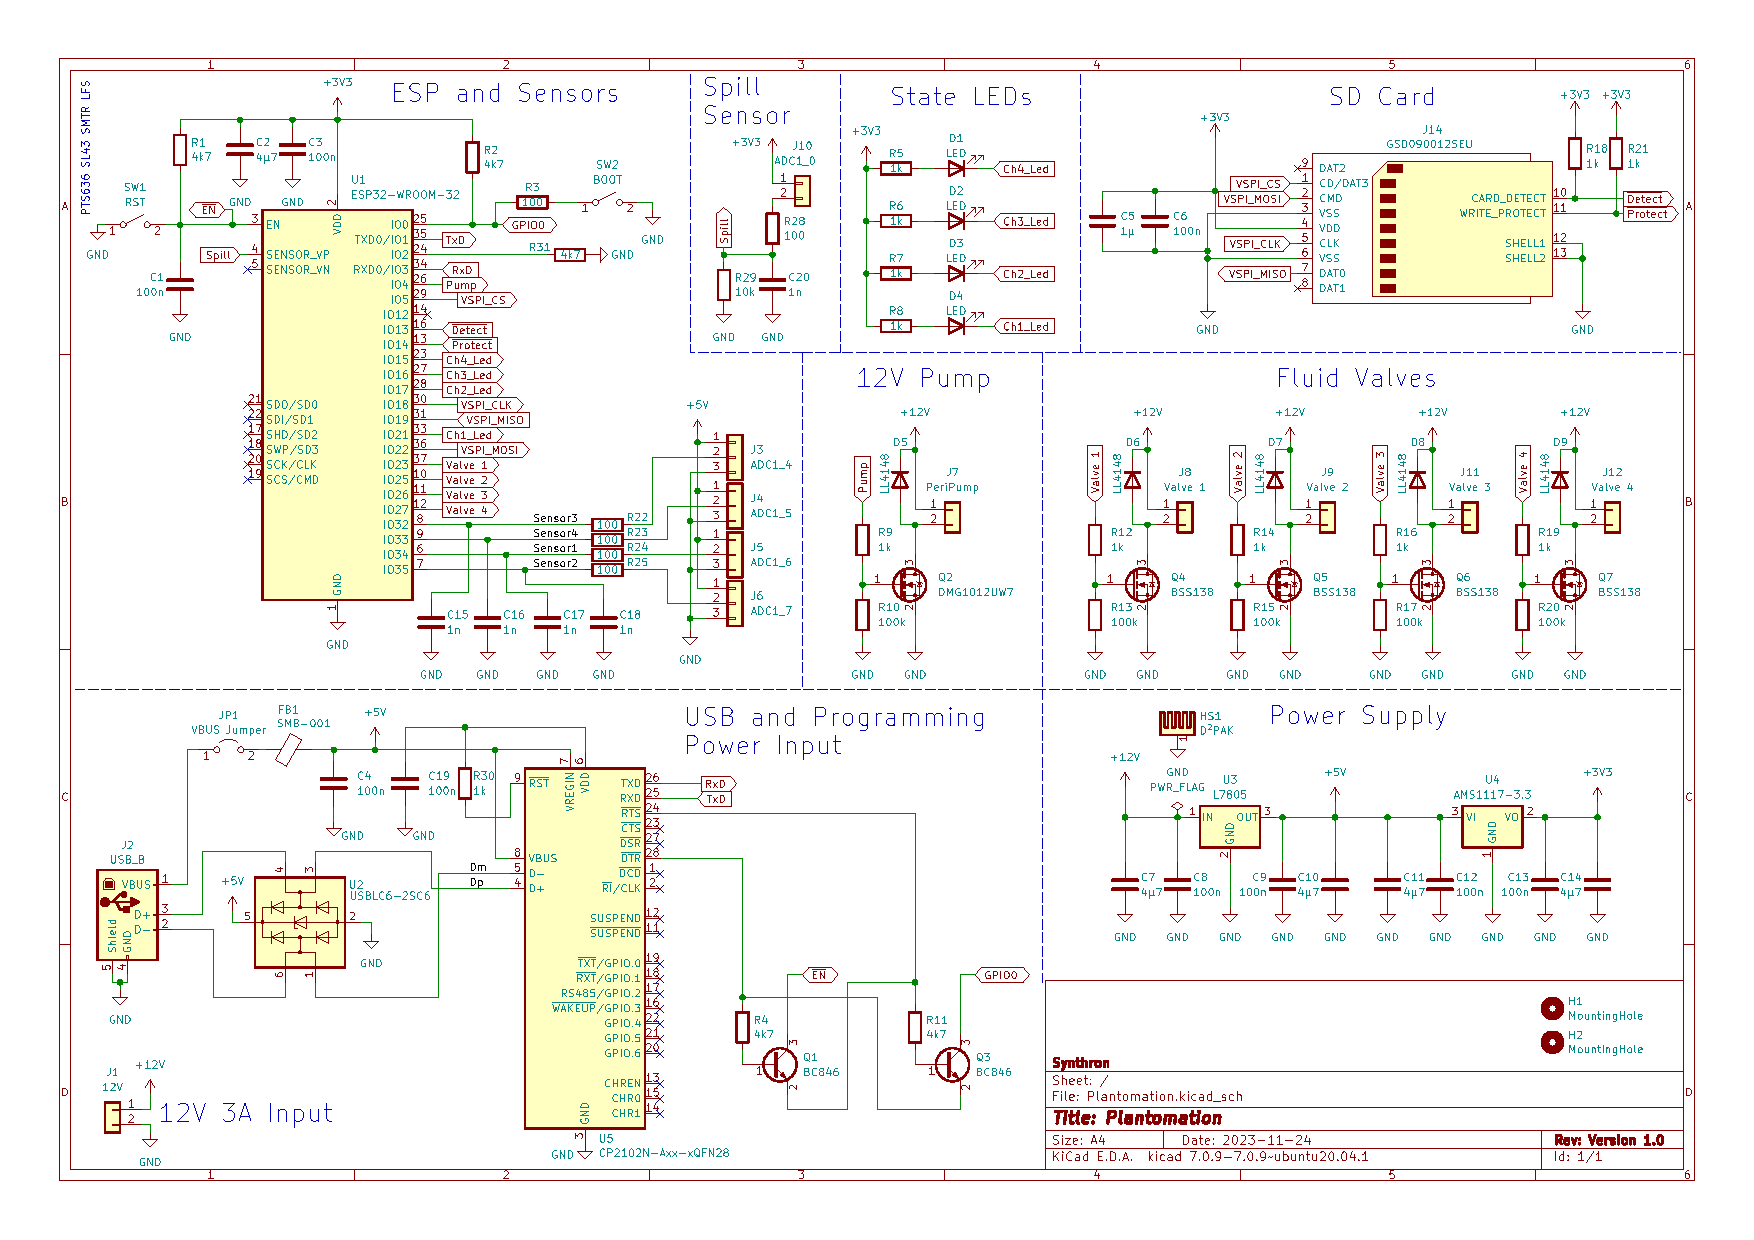
\includegraphics[angle=90,width=\textwidth]{../Hardware/Plantomation.pdf}

% --------------------------------------------------------------------
\end{document}